\documentclass{article}

\usepackage[preprint]{nips_2018}
% to avoid loading the natbib package, add option nonatbib:
% \usepackage[nonatbib]{nips_2018}

\usepackage[utf8]{inputenc} % allow utf-8 input
\usepackage[T1]{fontenc}    % use 8-bit T1 fonts
\usepackage{hyperref}       % hyperlinks
\usepackage{url}            % simple URL typesetting
\usepackage{booktabs}       % professional-quality tables
\usepackage{amsfonts}       % blackboard math symbols
\usepackage{nicefrac}       % compact symbols for 1/2, etc.
\usepackage{microtype}      % microtypography
\usepackage{amsmath}
\usepackage{float}
\usepackage{graphicx}
\usepackage{algorithm}
\usepackage{algpseudocode}
\usepackage{cleveref}       % this package must be loaded at the last
\usepackage{subcaption}


\title{Replication Report: Zero-shot Knowledge Transfer via Adversarial Belief Matching}

\author{
  Chun Hung Lin \\
  \texttt{chlin3@kth.se}
  \And
  Run Yan Tan \\
  \texttt{rytan@kth.se}
  \And
  Vivek Chalumuri \\
  \texttt{vivekc@kth.se}
}

\begin{document}
% \nipsfinalcopy is no longer used

\maketitle

\begin{abstract}

  This project is aimed to replicate the methods described in the paper \textit{Zero-shot Knowledge Transfer via Adversarial Belief Matching} \cite{micaelli2019zero}. We have reimplemnted all the major methods described in the paper from scratch using the information from the paper and the provided references. In order to offer an additional value to the Deep Learning community we have used \textit{Tensorflow} for our implementations unlike the pre-existing \textit{pyTorch} implementation provided by the authors. Our code  is available at: \url{https://gits-15.sys.kth.se/rytan/advanced-deep-learning-project}.

\end{abstract}

\section{Introduction}

Knowledge distillation as popularized by \cite{hinton2015distilling},  is a way to transfer knowledge from a cumbersome teacher model to a relatively simpler student model. However, the data used to train teachers might not always be available. Paper \cite{micaelli2019zero} proposes a novel method to train student networks from pre-trained teacher models without using any data. They achieve this by using an adversarial generator to find images where student fails to match the predictions of teacher and then use them to train the student. Their experiments claim a significant improvement by the proposed zero-shot method over traditional few-shot learning methods on simpler datasets like CIFAR-10 and SVHN. Moreover, they propose a metric to measure the degree of belief matching between the zero-shot student and the teacher model at the decision boundaries.

In this project we aim to reimplement the algorithms proposed by the authors, reproduce their experimental results and verify their claims. In this regard, we have reimplemented the wide-residual network \cite{zagoruyko2016wide} to train our teacher models, the knowledge distillation with attention transfer (KD+AT) training algorithm \cite{micaelli2019zero} for few-shot KD experiments, the zero-shot training algorithm \cite{micaelli2019zero}, and finally the transition algorithms \cite{micaelli2019zero} to compute transition curves between the networks and to measure the mean transition error (MTE). Similarly, we have used CIFAR-10 dataset for our main experiments so that we are able to compare with the results of the authors.

\section{Methods}\label{methods}

In order to address the replicability of the paper, we try to answer the following questions:

\begin{itemize}
    \item Can we reimplement the proposed algorithms from only information available in the paper?
    \item Is it possible to reproduce the results using the proposed zero-shot training algorithm?
    \item What are the sensitive points of the described methods and how can the proposed implementation be improved further?

\end{itemize}  In the following sections, we explain the algorithms for zero-shot training and transition curve computation, followed by our experiments, results and further discussion.
\subsection{Knowledge Distillation, Attention Transfer, and Few-Shot learning}

In traditional knowledge distillation, we train with real training data and minimize the KL divergence between the teacher logits and the student logits over the train data. In knowledge distillation with attention transfer (KD+AT), we use blockwise attention differences between the student and teacher as the extra loss term \cite{zagoruyko2016paying} to motivate the student to get closer to teacher. Finally, if it is a few-shot learning scenario, we follow the same procedure but this time training only with a fixed number of samples ($M$) per class from the train data instead of using the entire data. If $p^s$ and $p^t$ represent student and teacher logits, y represent onehot labels, and $T$ is the temperature of softmax. Knowledge distillation loss can be described as follows:

\begin{equation}
    L_{KD}=(1-\alpha)L_{CE}(p^s, y)+(2 \alpha T^2)D_{KL}(\frac{p^s}{T} || \frac{p^t}{T})
\end{equation}
$L_{CE}$ and $D_{KL}$ represent cross-entropy and KL divergence loss respectively.

% Zero-shot knowledge transfer
\subsection{Zero-shot Knowledge Transfer Algorithm}
We starts with a teacher model $T(x)$ which outputs probability vector $t$ for an input image $x$. $S(x;\theta)$ is the student network which outputs probability vector $s$. The authors use an adversarial generator $G(z;\phi)$ which produces pseudo images $x_p$ from a noise vector $z\sim N(0,I)$. The generator is then trained such that the forward KL divergence loss between the logits of teacher and student on the pseudo images is maximized, while the student is trained to minimize this loss. For student training, authors use Attention Transfer (AT) loss \cite{zagoruyko2016paying} along with KL divergence as the student and teacher usually have similar block structures. The losses for the generator $L_G$ and student $L_S$ can be described as follows:

\begin{equation}
    L_G=-D_{KL}(T(x_p) || S(x_p))
\end{equation}

\begin{equation}
    L_S=D_{KL}(T(x_p) || S(x_p))+\beta \sum^{N_L}_{l}{\left\|\frac{f(A_l^{(t)})}{\left\|f(A_l^{(t)})\right\|_2}-\frac{f(A_l^{(s)})}{\left\|f(A_l^{(s)})\right\|_2} \right\|}_2
\end{equation}

In the above equation, $A_l$ represents the activations of a block in the teacher or student network, $f(A_l)$ is the spatial attention map as introduced by \cite{zagoruyko2016paying}. Training scheme is explained in Algorithm \ref{algorithm1}. For every iteration in \textit{N}, we sample a random batch of noise \textit{z} which is used for $N_g$ gradient updates to generate a batch of psuedo images $x_p$ such that it minimizes $L_G$. We then use this same $x_p$ for $N_s$ gradient updates of student to match teacher and student logits. The authors use $N_s < N_g$ in order to give more time to the student to match teacher on $x_p$. Also if student is able to match the teacher, in the next iteration generator would be more compelled to generate images exploring different regions in the input space.

\subsection{Computing Transition Curves}
The transition curve shows how the student and teacher behave as we change the input data. The idea is to measure the difference in beliefs of the two networks at the decision boundaries. If we adversarially change the input such that the student's prediction $p_i^s$ on class $i$ decrease and prediction $p_j^s$ on class $j$ increase, then we want to find out how much the teacher's predictions on class $i$ and class $j$ change considering that both teacher and student initially predicted class $i$. Algorithm \ref{algorithm2} shows the method to compute the transition curve between two networks. To quantify this further, the authors introduced a metric called Mean Transition Error (MTE) which measures the absolute difference between $p_j^t$ and $p_j^s$ averaged over $K$ adversarial steps and $N_{test}$ images and $C-1$ classes. The authors claimed that the student trained by zero-shot matches the teacher's transition curves more closely compared to a student trained with the KD+AT method.
\begin{equation}
    MTE(nw_A,nw_B)=\frac{1}{N_{test}}\sum^{N_{test}}_{n}{\frac{1}{C-1}}\sum^{C-1}_{c}{\frac{1}{K}}\sum^{K}_{k}{\left|p_j^A-p_j^B\right|}
\end{equation}

\begin{minipage}{0.44\textwidth}
\begin{algorithm}[H]
    \centering
    \caption{Zero-Shot KT}\label{algorithm1}
    \begin{algorithmic}[1]
        \State \text{\textbf{pretrain}: $T(.)$}
        \State \text{\textbf{initialize}: $G(.;\phi)$}
        \State \text{\textbf{initialize}: $S(.;\theta)$}
        \For{$i=1,2....N$}
            \State $z\sim N(0,I)$
            \For{$i=1,2....N_g$}
                \State $x_p \gets G(z;\phi)$
                \State $L_G \gets -D_{KL}(T(x_p) || S(x_p))$
                \State $\phi \gets \phi-\eta\frac{\partial L_G}{\partial \phi}$
            \EndFor
            \For{$i=1,2....N_s$}
            \State $L_S \gets D_{KL}(T(x_p) || S(x_p)) + AT\_Loss$
            \State $\phi \gets \phi-\eta\frac{\partial L_S}{\partial \theta}$
            \EndFor
            \State decay $\eta$
        \EndFor
    \end{algorithmic}
\end{algorithm}
\end{minipage}
\hfill
\begin{minipage}{0.55\textwidth}
\begin{algorithm}[H]
    \centering
    \caption{Computing Transition Curves}\label{algorithm2}
    \begin{algorithmic}[1]
        \State \text{\textbf{pretrain}: $nw_A$}
        \State \text{\textbf{pretrain}: $nw_B$}

        \For{$x \in X_{test}$}
        \State $i_A\equiv$ class of $x$ according to $nw_A$
        \State $i_B\equiv$ class of $x$ according to $nw_B$
            \If{$i_A = i_B = i$}
            \State $x_0 \gets x$
                \For{$j \ne i$}
                \State $x_{adv} \gets x_0$
                    \For{$1,2,...,K$}
                    \State$y_A, y_B\gets nw_A(x_{adv}),nw_B(x_{adv})$
                    \State $x_{adv} \gets x_{adv}-\xi\frac{\partial L_{CE}(y_A,j)}{\partial x_{adv}}$
                    \State \textbf{save:} $y_A,y_B$
                    \EndFor
                \EndFor
            \EndIf
        \EndFor
    \end{algorithmic}
\end{algorithm}
\end{minipage}


\section{Experiments}\label{exp}

% Overview
\subsection{Experiment Overview}
We first replicate the knowledge distillation with different methods for CIFAR10 dataset. For the knowledge distillation method, we use the authors' zeroshot method and a finetuned zeroshot method with $M$ sample images per class. Also, we included few-shot knowledge distillation with attention transfer, training student from scratch as the baseline for comparsion.

After that, we replicate the experiment which aims to shows that different architecture teacher-student pairs performs better than others. In this experiment, we run three seeds and report the mean and standard deviation.

Moreover, we replicate the transitional curve and Mean Transition Error experiment and provided a computational efficient approximation method.

As we have limited computational resources, we only run three times with different seeds for the second experiment.

\subsection{Datset}

We used CIFAR-10 \cite{cifar10} dataset for all our major experiments which contains 32*32*3 images with 10 classes. Total 50K train and 10K test images are available in the dataset.

\subsection{Implementation Details}

For all our implementation, we have used tensorflow v1.14. We started with implementing our own wide-residual network \cite{zagoruyko2016wide} to train teacher models from scratch. For training, we have used the information provided in the paper, namely SGD with nesterov momentum. For the optimizer parameters, the momentum is 0.9, dampening is 0, and weight decay of $5\times10^{-4}$. \cite{zagoruyko2016wide} The initial learning rate of 0.1 was followed by decay factor of 0.2 at 30\%, 60\% and 80\% of the run. The authors mentioned that they used 80K training iterations but did not mention the batch size, therefore we obtained the batch size of 128 from the author's git repository for our own replication. A batch size of 128 results in 205 epochs. We used horizontal flip and random crop for data augmentation. \cite{zagoruyko2016wide} For KD+AT baselines we used the similar settings as the teacher training. We did most of our experiments with $M=200$ to compare with zero-shot just as the authors did. We use $\alpha=0.9$ and $T = 4$ for knowledge distillation loss calculations when the training labels are present. We noticed that attention transfer loss has been implemented differently by the authors. Instead of using an $L2$ as it is their implementation doesn't have the required square root over the mean vectors.

For zero-shot training, the generator details were not mentioned by the authors, so we used a generator architecture (around 1M parameters) which takes in a batch of noise vector of dimension 100 and outputs in a batch of 32 $\times$ 32 $\times$ 3 pseudo images. Generally, it is made up of 4 layers each with upsampling, convolutional, batch normalization and/or leaky ReLU layers. From the information in the paper for algorithm \ref{algorithm1}, we used $N=80$K, $N_g=1$, $N_s=10$ and $\beta=250$ for the attention loss. We used Adam optimizer with cosine annealing and initial learning rate $2\times10^{-3}$ for student. The learning rate of $1\times10^{-3}$ for the generator is not mentioned in the paper, therefore we obtained it from the author's git repository for our own replication.

For computing transition curves, we first replicated the authors' algorithm \ref{algorithm2}. Next, we realized that the algorithm can be improved by using batch to increase efficiency and also to help in sampling from the different classes. When perturbing images sampled from the test set, we perturb the image on a batch of images instead of a single image. A single batch of images contains only the images predicted as the same class initially. As we jitter the images to move from class i to j according the student network, we take the mean direction of the whole batch. As the cross-entropy function provided by tensorflow or pytorch will average the loss by the batch size. In actual implementation, we have to compensate this the batch size by multiply it back to the loss and use a small batch ($\leq$ 200) in order to have the similar behavior in algorithm \ref{algorithm2}. The method we purposed can be considered as an approimation method of the original one. Our final algorithm for computing transition curves is shown in algorithm \ref{algorithm3}.

\section{Results and Discussion}
% Exp part 1: replicate the knowledge distillation with different methods
For different knowledge distillation methods, the test accuracy performances are shown in Figure \ref{fig:KDMethodsPerformance}. Overall few-shot KD+AT performs better than training student from scratch and zeroshot with or without using real data performs better that few-shot KD+AT model. We got 80.14\% test accuracy for the zeroshot knowledge transfer method without using any real data. We also naively added training the student model with $M$ images per class in the zeroshot knowledge transfer method as the replication of the authors' few-shot version of the zeroshot model. We train the student model with real image right after training with pseudo images in a single loop. However, we got 76.27\% which is lower than the zeroshot model with no real data. The authors obtained a better performance with using the real images. Due to the time limitation, we did not try different training orders to obtain a result that with real data is better than without real data. It is confirmed that using real data actually make the student and generator model converge faster at the initial stage. The result is shown in Figure \ref{fig:ZeroshotMethodWWoRealImg}. However, early convergence could also be a cause of the model going to a sub optimal point.

Our teacher models trained over three seeds on different architectures of WRN\cite{zagoruyko2016wide} give us almost the same results as the teacher models used by the authors for their experiments. Table \ref{table:1} shows our results of zero-shot knowledge transfer between different WRN network pairs. Just like authors, we compare our zero-shot results with KD+AT at $M=200$. From table \ref{table:1}, we can see that student trained by zero-shot training proposed by the authors performs better than KD+AT student with 200 real samples per class. However, we observe that our results is a bit lower than the authors' result. We checked our implementation against the authors' implementation and found that they sampled with the same seed in each student training loop. With the use of batch normalization, the sampled images will be sightly different even using the same seed. As the result, it increases the performance of the student model just like image augmentation. Therefore, our replication results of the zeroshot model is about 2\% lower than the authors' results.
% Comment the below if not applicable
The pair of WRN-16-2 teacher and WRN-16-1 student has a significant drop in zeroshot model comparing with the authors' result. We got 71.29\% $\pm$ 2.74\% while they obtained 82.44\% $\pm$ 0.21\%. Our best test accuracy of this pair in zeroshot model among the three runs is 75.06\% which is close to the authors' results while the other runs are far from that. We have no clue that why there is such a huge difference yet our other zeroshot model pair performances are consistent. Changing the teacher from WRN-16-2 to WRN-40-1 gains a huge difference while the authors' results does not show this trend.

We notice that training mode of generator and student are critical in zero-shot training. Both student and generator need to be in training mode in both phases of generator and student training. Due to the presence of batch-norm layers in the networks they tend to behave differently in train and evaluation modes. So, if we place either the student in evaluation mode during generator training or generator in evaluation mode during student training, we will not get the consistent training behaviour. This results in pseudo images in generator training and ones used in student training to belong to different regions of input space.

% Double check this claim after Nov-1
Gradient-clipping is another tool we found very useful for zero-shot training. Without gradient-clipping we found that the generator loss as well as the student loss blow up. The generator creates training samples that the teacher and student cannot classify with confident. These generated samples are probably irrelevant to the data that the teacher can classify. As the result, we cannot use these generated pseudo images to transfer knowledge from the teacher to the student.

% Sampling from the generative model.
We sample images from the generative models saved during the training phase and the results are shown in Figure \ref{fig:GenerativeModelsSamples}.
We hold the same conclusion as the authors' that at the initial the psuedo images are coarse but become reasonably diverse at the later training epochs.
We also noticed that the color of the psuedo images is unrealistic (colors are evenly distributed) at the early training stage and it becomes realistic
at the later stage like more green, grey, and blue color.

% Transitional curve
We set WRN-40-2 as the teacher model and WRN-16-1 as the student model to replicate the authors' results on Transition Curve and Mean Transition Error (MTE). For training student model, we have zero shot training, few shot KD+AT, and standard knowledge distillation without attention loss using whole training set. We used both algorithm \ref{algorithm2} and algorithm \ref{algorithm3}. We used 100 adversarial steps ($K = 100$) and the learning rate ($\xi = 1$). The replication result is placed in Table \ref{table:2}. We can see that zero-shot student has the lowest transition error as the student trained with teacher's decision boundary marked by the generated training samples. The second lowest is the student distilled with full training set and the highest is the student distilled with the KD+AT method. This is likely because whether the student uses partial or full training set would result in different decision boundaries from the teacher. Using less training data gives student more degree of freedom to have different decision boundaries.

The transition curves are plotted in Figure \ref{fig:TCurvesWONormalize}.
We found that the transition curve of zero-shot student is close to the authors' result while others are not. It is because when we apply Batch Gradient Descent, the gradient for perturbing the images is the mean direction over the whole batch. We could obtain images that we cannot move from class i to j by jittering the images with the mean direction gradient. In order to have a fair comparison between different models, we introduce Relative Mean Transition Error which is the Mean Transition Error divided by the maximum value of $p^{A}_j$ and $p^{B}_j$ which are averaged over test samples and classes. In other words, we normalize the transition curves such that the maximum value of the curves is 1. We see it justifiable as we would like to focus on the images that are possible to move from class i to j from the image perturbation and we want to have this metric comparable across experiments. The Relative Mean Transition Error results are shown in Table \ref{table:2} and Figure \ref{fig:TCurvesWNormalize}. Comparing tables 2 and 3, we obtain similar conclusion for our relative error.

For the computation efficiency, algorithm \ref{algorithm2} typically takes 6 hours with NVIDIA Tesla P100 GPU while algorithm \ref{algorithm3} takes only 10 minutes for the same configuration of adversarial steps ($K$).

\begin{table}[h!]
\begin{tabular}{cccccc}
\begin{tabular}[c]{@{}c@{}}Teacher\\ (\# params)\end{tabular} & \begin{tabular}[c]{@{}c@{}}Student\\ (\# params)\end{tabular} & \begin{tabular}[c]{@{}c@{}}Teacher\\ scratch\end{tabular} & \begin{tabular}[c]{@{}c@{}}Student\\ scratch\end{tabular} & \begin{tabular}[c]{@{}c@{}}KD + AT\\ (M = 200)\end{tabular} & \begin{tabular}[c]{@{}c@{}}Zero-Shot\\ (M = 0)\end{tabular} \\
\hline
WRN-16-2(0.7M) & WRN-16-1(0.2M) \vline & 93.91 $\pm$ 0.08 & 91.63 $\pm$ 0.26 & 81.41 $\pm$ 0.76 & 71.29 $\pm$ 2.74\\
WRN-40-1(0.6M) & WRN-16-1(0.2M) \vline & 93.50 $\pm$ 0.12 & 91.63 $\pm$ 0.26 & 78.69 $\pm$ 0.44 & 78.48 $\pm$ 1.81\\
WRN-40-2(2.2M) & WRN-16-1(0.2M) \vline & 94.55 $\pm$ 0.05 & 91.63 $\pm$ 0.26 & 80.23 $\pm$ 0.56 & 80.91 $\pm$ 0.69\\
WRN-40-1(0.6M) & WRN-16-2(0.7M) \vline & 93.50 $\pm$ 0.12 & 93.91 $\pm$ 0.08 & 82.19 $\pm$ 0.35 & 80.69 $\pm$ 2.70\\
WRN-40-2(2.2M) & WRN-16-2(0.7M) \vline & 94.55 $\pm$ 0.05 & 93.91 $\pm$ 0.08 & 78.30 $\pm$ 0.40 & 87.18 $\pm$ 0.34\\
WRN-40-2(2.2M) & WRN-40-1(0.6M) \vline & 94.55 $\pm$ 0.05 & 93.50 $\pm$ 0.12 & 78.74 $\pm$ 0.76 & 84.95 $\pm$ 0.37\\
\end{tabular}
\caption{Comparison between KD+AT at $M=200$ and the Zero-Shot method for different WRN teacher-student pairs on CIFAR-10. Scratch results are reported as mean and std over 3 seeds.}
\label{table:1}
\end{table}

\begin{table}[h] % non-relative
    \centering
    \begin{tabular}{|c|c|c|}
    \hline
    Zero-Shot & KD+AT & Normal KD\\ \hline
    0.22      & 0.66  & 0.5 \\ \hline
\end{tabular}
\caption{MTE between Zero-Shot student and teacher compared with KD+AT  and just KD student-teacher pairs on CIFAR-10. Results are obtained through the authors' algorithm \ref{algorithm2} and are consistent with authors' results showing zero-shot student's greater match to teacher compared to the KD+AT method and the normal knowledge distillation method.}
\label{table:2}
\end{table}

\begin{algorithm}[]
    \centering
    \caption{Computing Transition Curves with Minibatch}\label{algorithm3}
    \begin{algorithmic}[1]
        \State \text{\textbf{pretrain}: $nw_A$}
        \State \text{\textbf{pretrain}: $nw_B$}
        \State \text{\textbf{initialize}: predClassList}
        \State \text{\textbf{initialize}: xList}
        \For{$x \in X_{test}$}
            \State $i_A\equiv$ class of $x$ according to $nw_A$
            \State $i_B\equiv$ class of $x$ according to $nw_B$
            \If{$i_A = i_B = i$}
                \State append(xList, $x$)
                \State append(predClassList, $i$)
            \EndIf
        \EndFor

        \\ \\
        // sort the saved test set by the predicted class
        \State index $\gets$ argsort(predClassList)
        \State predClassList $\gets$ apply(predClassList, index)
        \State xList $\gets$ apply(xList, index)

        \\ \\
        // split the same prediction classes into batches
        \\
        // the first batch should be all predicted as class 0, etc
        \State xBatchByClass, classes $\gets$ splitToBatch(xList, predClassList)

        \\ \\
        // do perturbation
        \For{$x, i \in \text{xBatchByClass}, \text{classes}$}
            \State $x_0 \gets x$
            \For{$j \ne i$}
                \State $x_{adv} \gets x_0$
                \For{$1,2,...,K$}
                    \State$y_A, y_B\gets nw_A(x_{adv}),nw_B(x_{adv})$
                    \State $x_{adv} \gets x_{adv}- \xi\frac{\partial L_{CE}(y_A,j)}{\partial x_{adv}}$
                    \State \textbf{save:} $y_A,y_B$
                \EndFor
            \EndFor
        \EndFor

    \end{algorithmic}
\end{algorithm}

\begin{table}[h] % relative
    \centering
    \begin{tabular}{|c|c|c|}
    \hline
    Zero-Shot & KD+AT & Normal KD\\ \hline
    0.22      & 0.58  & 0.40 \\ \hline
\end{tabular}
\caption{Relative MTE between Zero-Shot student and teacher compared with KD+AT  and just KD student-teacher pairs on CIFAR-10. Results are obtained through our minibatch algorithm \ref{algorithm3} and are close to Table \ref{table:2} (slightly lower for KD+AT and Normal KD).}
\label{table:3}
\end{table}

\begin{figure}
    \centering
    \begin{minipage}{.48\textwidth}
        \centering
        \includegraphics[width=\linewidth]{Plots/method_cmp.pdf}
        \caption{
            The performance of zeroshot knowledge transfer model for a WRN-40-2 teacher
            and WRN-16-1 student on CIFAR-10 dataset against different numbers of
            images per class.
            }
        \label{fig:KDMethodsPerformance}
    \end{minipage}%
    \hfill
    \begin{minipage}{.48\textwidth}
        \centering
        \includegraphics[width=\linewidth]{Plots/cmp_zero_wwo_real_data.pdf}
        \caption{
            The lose against epoch plot for a WRN-40-2 teacher and WRN-16-1 student
            on CIFAR-10 dataset with or withour using limited amount of real data.
            The number of image per class is 100.
        }
        \label{fig:ZeroshotMethodWWoRealImg}
    \end{minipage}
\end{figure}

% The generative samples
\begin{figure}
    \centering
    \includegraphics[width=0.8\linewidth]{Plots/cifar10-generator-samples.pdf}
    % \caption{Images sampled from the generative model at different epochs}
    \caption{
        Pseudo images sampled from the generator at different epochs.
        We use the generator from the WRN-40-2 teacher and WRN-16-1 student zeroshot training.
        with the random seed is 45.}
    \label{fig:GenerativeModelsSamples}
\end{figure}

\begin{figure}[h!]
  \centering
  \begin{subfigure}[b]{0.32\linewidth}
    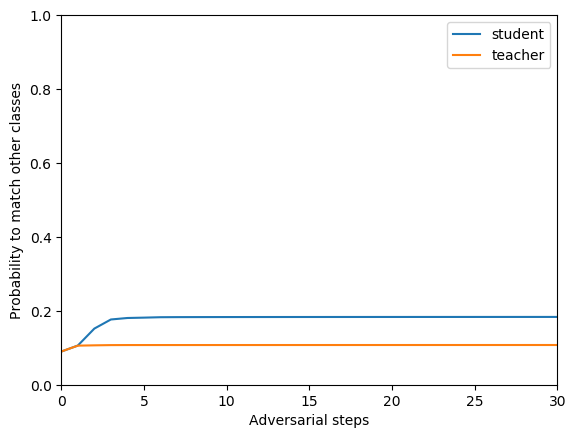
\includegraphics[width=\linewidth]{Plots/normalkd.pdf}
     \caption{Normal KD Student}
  \end{subfigure}
  \begin{subfigure}[b]{0.32\linewidth}
    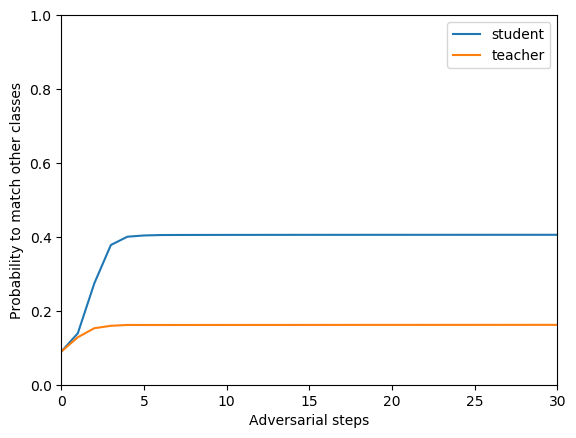
\includegraphics[width=\linewidth]{Plots/fewshot.pdf}
    \caption{Few-Shot ($M=200$) Student}
  \end{subfigure}
  \begin{subfigure}[b]{0.32\linewidth}
    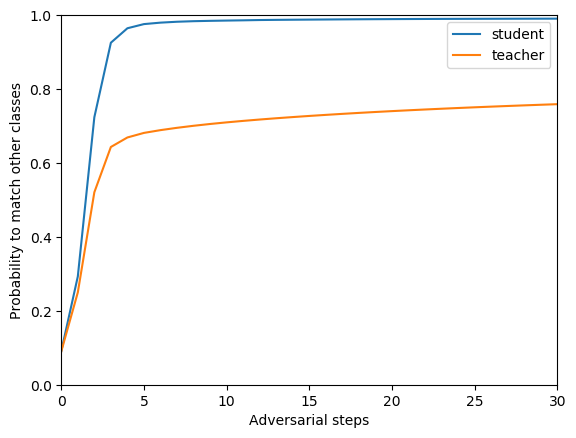
\includegraphics[width=\linewidth]{Plots/zeroshot.pdf}
    \caption{Zero-Shot Student}
  \end{subfigure}
  \caption{Average Transition Curves without normalization over 9 classes for CIFAR-10 with our algorithm \ref{algorithm3}.}
  \label{fig:TCurvesWONormalize}
\end{figure}

\begin{figure}[h!]
  \centering
  \begin{subfigure}[b]{0.32\linewidth}
    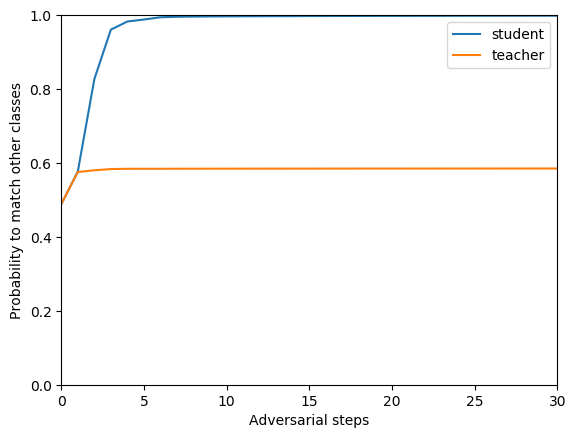
\includegraphics[width=\linewidth]{Plots/renormal_normalkd.pdf}
     \caption{Normal KD Student}
  \end{subfigure}
  \begin{subfigure}[b]{0.32\linewidth}
    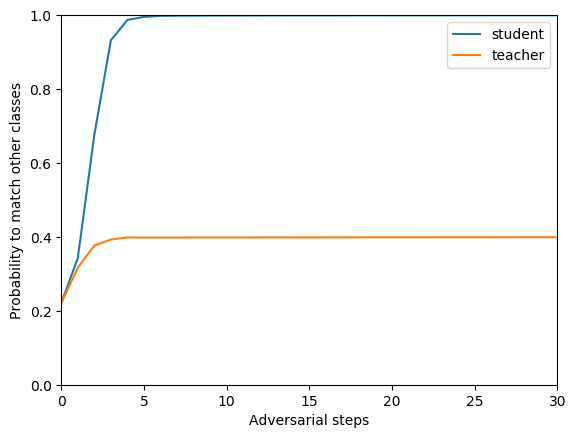
\includegraphics[width=\linewidth]{Plots/renormal_fewshot.pdf}
    \caption{Few-Shot ($M=200$) Student}
  \end{subfigure}
  \begin{subfigure}[b]{0.32\linewidth}
    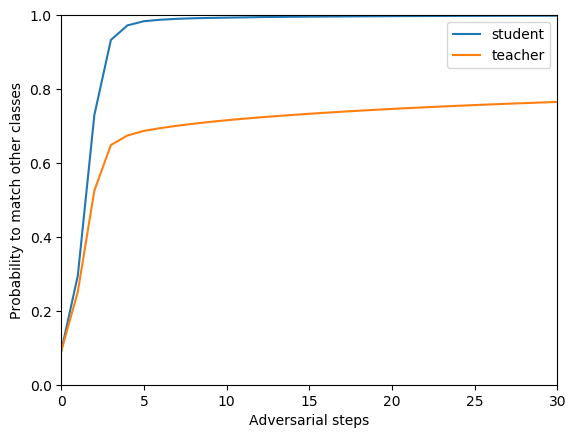
\includegraphics[width=\linewidth]{Plots/renormal_zeroshot.pdf}
    \caption{Zero-Shot Student}
  \end{subfigure}
  \caption{Average Transition Curves with normalization over 9 classes for CIFAR-10 with our algorithm \ref{algorithm3}.}
  \label{fig:TCurvesWNormalize}
\end{figure}

\section{Ablation}

We performed an ablation test on the attention transfer (AT) loss because we are very curious about how making the student activations close to the teacher activations would help the student to learn. We want to ask the question - how different will the student be if we do not use the AT loss? The result is that the AT loss might not be a very important loss because by removing attention loss, the trained student's test accuracy is 78.93\% compared to our zero-shot student test accuracy of 80.94\% (both using WRN-40-2 teacher and WRN-16-1 student). Therefore, looking from the opposite point of view, without AT loss, the zero-shot learning as proposed in this paper may be slightly lower (lower by 2.01\% as shown in our ablation experiment), but it would still be successful. However, we would still recommend testing with more model pairs to verify if this conclusion is the same for other model pairs.



\section{Conclusions}

We have successfully reimplemented all of the authors' major methods and experiments in \textit{TensorFlow}, which is a different deep learning framework than the \textit{PyTorch} framework that they used. Due to time constraints, we limited our experiments to CIFAR-10 dataset but we performed all the major experiments. We reimplemented all of authors' algorithms and verified the zero-shot performance and compared it with few-shot KD+AT student training. We improved upon the authors transition curve computation algorithm \ref{algorithm2} and increased its computational efficiency by using mini-batches algorithm \ref{algorithm3}. Additionally, we also used another data set - the grayscale Fashion-MNIST \cite{fashionMnist} data to transfer knowledge from scratch from a WRN-40-2 teacher to a WRN-16-1 student with a test accuracy of 94.48\%. Furthermore, we achieved 77.15\% accuracy with zero-shot training on this data set. We also performed an ablation experiment by removing the attention loss and training a student with a test accuracy that is very close to the student trained with attention loss (2.01\% difference). We recommend future work to experiment with more complex data sets and diverse network architectures to find out their impact on zero-shot learning.


\medskip
% \small
% \pagebreak
\bibliographystyle{unsrt}
\bibliography{references}

\end{document}
